\section{Reti a connessione diretta - Data Link Layer}
Abbiamo dei nodi connessi tra di loro attraverso dei link di connessione, ne possiamo avere di diverso tipo: cavi elettrici, fibre ottiche, connessioni via etere, ecc.
Ci serve per tanto dell' hardware che permetta di codificare i bit che vogliamo trasmettere in un segnale elettrico/luminoso/elettromagnetico in modo da poter essere trasportato dal link fisico.
Questa codifica (\emph{encoding}) è eseguita da un trasmettitore, all' altro capo del link vi deve essere invece un ricevitore che effettui la decodifica (\emph{decoding}).
Una semplice codifica che possiamo immaginare attraverso un link in rame può essere:
\begin{itemize}
    \item livello alto di tensione: 1 logico
    \item livello basso di tensione: 0 logico
\end{itemize}
\begin{figure}[H]
    \centering
    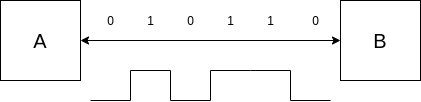
\includegraphics[width=300px]{images/3_Reti_connessione_diretta/encoding.png}
\end{figure}
tuttavia ce ne possono essere diverse in base al mezzo, alla velocità da usare, ecc, ma sono tutte questioni che riguardano la teoria dei segnali e non le reti in se per se.

Essendo la trasmissione bidirezionale ogni capo della connessione è dotato di un trasmettitore ed un ricevitore, lo chiamiamo ricetrasmettitore (\emph{transceiver}).

Ovviamente il canale di trasmissione non è ideale, il che comporta problemi di attenuazione (il segnale perde di potenza durante il percorso), disturbi, rumore ed altro che possono portare il segnale a cambiare in maniera importante, modificando quindi il contenuto delle informazioni che trasporta.

Anche la campionatura del segnale è problematica: per campionare al meglio sarebbe necessario campionare sul picco, ma non abbiamo la certezza di quando il picco avvenga.
Se i due endpoint non sono sincronizzati un capo non sa quando è il picco dell' altro capo, anche se fossero sincronizzati i circuiti del clock non sono perfettamente identici quindi il drift li porterebbe fuori sincro in poco tempo.

E' utile definire l' error rate:
$$ \text{error\_rate} = \frac{\text{bit\_errati}}{\text{bit\_trasmessi}} $$

Il Data Link Layer è il layer dello stack ISO/OSI che si occupa di fornire l' astrazione di un canale affidabile.
Non importa cosa c' è al livello fisico, l' importante è che i dati vengano trasmessi bene tra due endpoint connessi in maniera diretta.



\subsection{Servizi del data-link layer}
Per ottenere l' affidabilità il data-link layer porta avanti alcune politiche.

\subsubsection{Framing}
Dato un error\_rate piccolo a piacere, se trasmetto tanti bit avrò sempre qualche bit che non arriva a destinazione in maniera corretta.
Per risolvere possiamo dividere il datagramma intero in dei \emph{frame} più piccoli ed aggiungervi un \emph{header} ed un \emph{trailer}.
\begin{figure}[H]
    \centering
    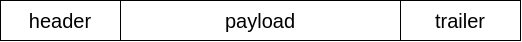
\includegraphics[width=250px]{images/3_Reti_connessione_diretta/frame.png}
\end{figure}

\subsubsection{Error detection \& correction}
Si occupa di capire se ci sono degli errori ed eventualmente correggerli.
Si applicano alcuni algoritmi che permettono di dire quale bit è arrivato in maniera errata e quindi flipparlo.
Questi algoritmi tuttavia sono affidabili solo per pochi bit errati ed a volte sono troppo pesanti in termini di bit aggiuntivi da inserire nel frame.

\subsubsection{Trasmissione dati affidabile}
Un' altra tecnica utilizzata è quella tramite acknowledge e ritrasmissione: quando ho ricevuto un frame lo segnalo, se qualche frame mi manca o è danneggiato lo chiedo nuovamente.
In fine riordino i frame per ottenere il datagramma intero.

\subsubsection{Flow control}
Permette di gestire la velocità con la quale inviare i dati sul media, questo è comodo qualora si interfaccino hardware diversi che non hanno la stessa velocità massima.

\subsubsection{Half-duplex e full-duplex}
Permette di negoziare, tramite il tipo di mezzo, se la connessione deve essere:
\begin{itemize}
    \item half-duplex: comunicazione bidirezionale ma uno per volta
    \item full-duplex: comunicazione bidirezionale e simultanea
\end{itemize}

\subsubsection{Implementazione}
Il data-link layer è implementato principalmente in hardware all' interno della Network Interface Card (NIC) in quanto deve interfacciarsi con il link fisico, tuttavia altre componenti, quelle più ad alto livello possono essere implementate interamente in software.

\subsection{Error detection}
L' algoritmo generico di error detection prevede che il trasmettitore aggiunga ai dati dei bit R ridondanti utilizzati dal ricevitore per controllare che i dati siano arrivati correttamente.
Questi bit R si aggiungono alla fine in modo che siano generati contestualmente alla trasmissione \emph{on-the-fly} ed il controllo possa avvenire durante la ricezione.
Ovviamente durante la trasmissione possono corrompersi sia i bit D che i bit R, supponiamo quindi che il ricevitore ottenga D' ed R': usa lo stesso algoritmo del trasmettitore che a partire dai bit D' genera i bit ridondati, li compara ai bit R' ricevuti ed agisce di conseguenza se sono diversi.

La error detection non è affidabile al 100\%, possono esserci alcuni casi limite dei vari algoritmi che non permettono di rilevare correttamente gli errori.
In genere aumentare il numero di bit R porta ad una migliore detection ma anche ad un maggiore numero di bit, non di dato, da inviare.

\subsubsection{Parity checking}
Si aggiunge in coda al messaggio un singolo bit di parità, questo bit si sceglie in modo da rendere pari il  numero di 1 all' interno del blocco, nella parità pari, oppure per rendere il conteggio dispari, nella parità dispari.
Questo metodo è usato per brevissimi spostamenti, ad esempio quelli memoria-CPU perché è poco affidabile, infatti riesce a rilevare il cambiamento di un singolo bit, ma se ve ne sono due modificati allora il bit di parità è corretto pur non essendolo il campo dati.

In hardware si può implementare tramite lo XOR/XNOR dei bit del campo dati.
\begin{figure}[H]
    \centering
    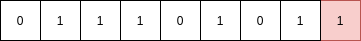
\includegraphics[width=200px]{images/3_Reti_connessione_diretta/parity_checking.png}
\end{figure}

\subsubsection{Checksum}
Si splitta il pacchetto in blocchi da 16 bit, li si tratta come interi e si esegue la somma bit a bit (complemento ad 1) di tutti i gruppi.
Il risultato di questa somma è detto \emph{checksum} e lo aggiungo in coda al pacchetto oppure in un campo ben preciso se il protocollo lo prevede (ad esempo il TCP usa questo algoritmo ed ha un campo del pacchetto apposito).
Il ricevitore ovviamente esegue la stessa somma, controlla con il valore ricevuto, se non matchano c'è la certezza che ci sia stato un errore durante la trasmissione.
Anche in questo caso non si può avere la certezza al 100\% che se i valori matchano allora i dati ricevuti sono corretti.

\subsubsection{Cyclic redundancy check - CRC}
Questo algoritmo è largamente utilizzato all' interno dei vari protocolli di data link (ad esempio Ethernet, 802.11 WiFi, ecc).
Vede il blocco di dati $D$ come un unico numero, si sceglie un numero di $r+1$ bit e lo si chiama $G$ (\emph{generatore}), scelgo opportunamente gli $r$ bit di parità e li chiamo $R$, li scelgo in modo che la concatenazione $<D, R>$ sia divisibile per $G$ nell' aritmetica modulo 2.
Quando il ricevitore riceve il numero prova ad eseguire la divisione per $G$, se il resto non è nullo ci sono stati degli errori nella trasmissione.
Questo algoritmo riesce a trovare i burst di errori con lunghezza minore di $r+1$ bit.

Si noti che il generatore $G$ deve essere comune a tutti e due gli endpoint, per far ciò si può prevedere un valore fisso all' interno del protocollo oppure negoziarne uno alla prima connessione.

Per trovare $R$ opportuno si deve risolvere questa equazione:
$$ D \cdot 2^{r} \oplus R = n \cdot G $$
$$ D \cdot 2^{r} = n \cdot G \oplus R $$
se dividiamo $D \cdot 2^r$ per $G$ il resto è uguale ad $R$:
$$ R = resto\left( \frac{D \cdot 2^r}{G} \right) $$

\subsection{Forward error correction}
Alcuni algoritmi oltre a mostrare che ci sono stati errori permettono di correggerli se sono in un giusto numero.

\subsubsection{Two-dimensional bit parity}
Si aggiungono al messaggio un bit di parità per ogni riga ed uno per ogni colonna ed incrociando i bit di parità sbagliati si trova il bit errato:
\begin{table}[ht!]
    \centering
    \begin{tabular}{c c c | c}
        $d_{1,1}$ & ... & $d_{1,j}$ & $d_{1,j+1}$ \\
        $d_{2,1}$ & ... & $d_{2,j}$ & $d_{2,j+1}$ \\
        ... & ... & ... & ... \\
        $d_{i,1}$ & ... & $d_{i,j}$ & $d_{i,j+1}$ \\
        \hline
        $d_{i+1,1}$ & ... & $d_{i+1,j}$ & $d_{i+1,j+1}$ \\
    \end{tabular}
\end{table}
Questo algoritmo prevede di introdurre quindi $i + j + 1$ bit di parità.

\subsection{Reliable data transfer}
Vogliamo creare l' astrazione di un trasporto dati affidabile: il layer in alto chiama una procedura che si occupa di inviare i dati ed essere certo che siano arrivati in maniera corretta, così come dall' altra parte essere sicuri che i dati ricevuti siano corretti.
Le interfacce che offrono questa astrazione sono:
\begin{itemize}
    \item \emph{rdt\_send}: procedura chiamata dal layer superiore per inviare dati
    \item \emph{deliver\_data}: procedura chiamata dal data link per consegnare i dati al layer superiore
\end{itemize}
Il data-link layer invece sfrutta le seguenti primitive messe a disposizione dal layer fisico:
\begin{itemize}
    \item \emph{udt\_send}: chiamata per inviare un pacchetto di dati su un canale non affidabile
    \item \emph{rdt\_rcv}: chiamata dal layer fisico quando arriva un nuovo pacchetto sul canale
\end{itemize}

Implementiamo un protocollo per affinamenti successivi ed usiamo il formalismo degli automi a stati finiti per descriverne il comportamento.


\subsubsection{RDT 1.0: rdt su un canale affidabile}
Su un canale affidabile non abbiamo errori durante la trasmissione e non abbiamo perdita di pacchetti, la situazione è semplicemente rappresentabile:
\begin{figure}[H]
    \centering
    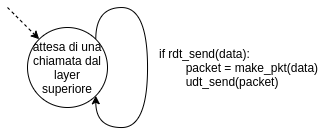
\includegraphics[width=200px]{images/3_Reti_connessione_diretta/rdt_1.0_sender.png}
    \caption{RDT 1.0 sender}
\end{figure}
Siamo sempre in attesa di una chiamata dal layer superiore, quando arriva una chiamata prendiamo i dati, prepariamo il pacchetto e lo spediamo sul canale.

\begin{figure}[H]
    \centering
    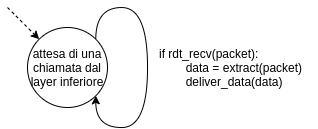
\includegraphics[width=200px]{images/3_Reti_connessione_diretta/rdt_1.0_receiver.png}
    \caption{RDT 1.0 receiver}
\end{figure}
Siamo sempre in attesa di una chiamata dal layer inferiore, quando arriva un pacchetto lo prendiamo, estraiamo i dati che vi sono contenuti all' interno e lo consegnamo al layer superiore.


\subsubsection{RDT 2.0: canale che può flippare i bit}
Introduciamo ora un canale che durante la trasmissione possa flippare alcuni bit presenti nel pacchetto.
Ci serve quindi un meccanismo di error detection (CRC o checksum in base al layer sul quale stiamo lavorando) per capire quando gli errori ci sono stati, ci serve poi anche un metodo per aggiustare la situazione.
Introduciamo quindi i concetti di \emph{acknowledgement} - ACK, con il quale il ricevitore notifica al trasmettitore l' avvenuta ricezione del pacchetto corretto e \emph{negative acknowledgement} - NAK, con il quale il ricevitore notifica al trasmettitore di aver ricevuto il pacchetto corrotto e ne richiede la ritrasmisione.

Stiamo quindi implementando una forma di Automatic Repeat reQuest - ARQ protocol.

\begin{figure}[H]
    \centering
    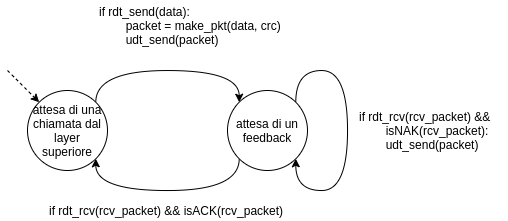
\includegraphics[width=300px]{images/3_Reti_connessione_diretta/rdt_2.0_sender.png}
    \caption{RDT 2.0 sender}
\end{figure}
Si attende una chiamata dal layer superiore, quando avviene si costruisce il pacchetto e lo si invia sul canale.
Si rimane quindi in attesa di un feedback, quando arriva se è positivo si torna in attesa di una chiamata dal layer superiore, se è negativo invece si reinvia il pacchetto e si torna in attesa di un feedback.

\begin{figure}[H]
    \centering
    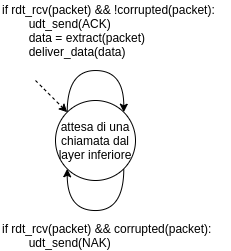
\includegraphics[width=150px]{images/3_Reti_connessione_diretta/rdt_2.0_receiver.png}
    \caption{RDT 2.0 receiver}
\end{figure}
Si attende l' arrivo di un pacchetto, quando arriva si controlla il suo stato, se non risulta corrotto allora si invia un ACK, si estraggono i dati e li si inviano al layer superiore, dopodiché si torna in attesa, se invece risulta corrotto si invia un NAK, si butta via il pacchetto e si ritorna in attesa.

Questo protocollo è basato sulla politica di \emph{stop-and-wait} cioè si invia un pacchetto e si aspetta per una risposta prima di fare qualsiasi cosa, vedremo più avanti che questo approccio è poco furbo in quanto si perde tanto tempo in attesa ma per adesso rimaniamo con questa logica.


\subsubsection{RDT 2.1: gestione degli errori sugli ACK/NAK}
Il protocollo precedente ha una falla importante: non abbiamo la certezza che ACK e NAK vengano trasmessi correttamente, essendo trasferiti sullo stesso canale non affidabile potrebbero arrivare in maniera errata, come potrebbero non arrivare.
Inoltre dato che c'è di mezzo una ritrasmissione c'è da accertarsi che i pacchetti che consegnamo al layer superiore non siano duplicati!
Per gestire i duplicati possiamo aggiungere al pacchetto un numero di sequenza, per protocolli stop-and-wait basta un solo bit di sequenza.
\begin{figure}[H]
    \centering
    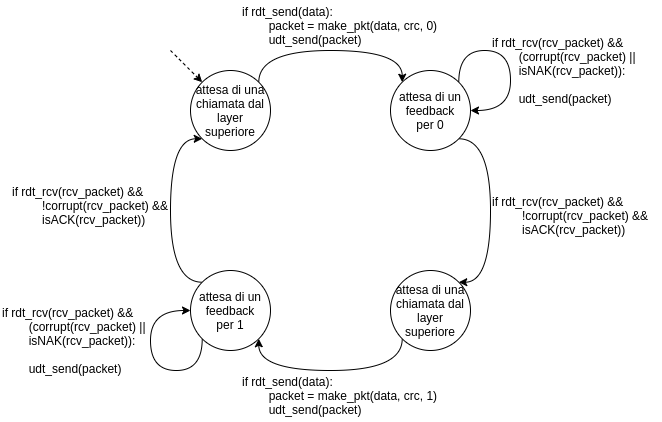
\includegraphics[width=340px]{images/3_Reti_connessione_diretta/rdt_2.1_sender.png}
    \caption{RDT 2.1 sender}
\end{figure}
All' arrivo di una richiesta costruiamo il pacchetto con sequence\_number a 0, lo inviamo, aspettiamo un feedback.
Se il feedback è negativo allora re-inviamo il messaggio, altrimenti ci portiamo in attesa della prossima richiesta.
Quando arriva una seconda richiesta costruiamo un nuovo pacchetto con sequence\_number ad 1, lo inviamo e ci mettiamo in attesa del feedback.
Quando arriva un feedback se è positivo torniamo in attesa di una richiesta, altrimenti rispediamo il pacchetto rimettendoci in attesa del feedback.

\begin{figure}[H]
    \centering
    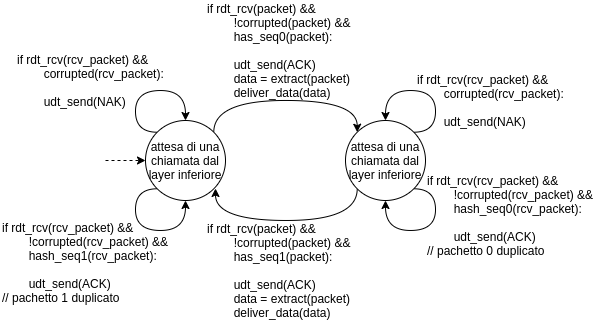
\includegraphics[width=340px]{images/3_Reti_connessione_diretta/rdt_2.1_receiver.png}
    \caption{RDT 2.1 receiver}
\end{figure}
All' arrivo di un pacchetto:
\begin{itemize}
    \item se non è corrotto ed ha sequence\_number 0: estraggo i dati e li consegno al layer superiore, invio un ACK e mi metto in attesa di un pacchetto con sequence\_number 1
    \item se è corrotto: invio un NAK
    \item se non è corrotto ma ha sequence\_number 0: invio un ACK e butto via il pacchetto in quanto siamo in caso di duplicati
\end{itemize}
stessa cosa per l' attesa del pacchetto con sequence\_number 1.


\subsubsection{RDT 2.2: protocollo NAK-free}
Possiamo evolvere il protocollo precedente eliminando i NAK ed eseguendo tutto tramite ACK.
Per fare ciò usiamo gli ACK aggiungendo il sequence\_number del pachetto di cui si sta confermando la corretta ricezione.
Il trasmettitore invece quando si vede arrivare un ACK con sequence\_number diverso dall' ultimo inviato re-invia il pacchetto.
\begin{figure}[H]
    \centering
    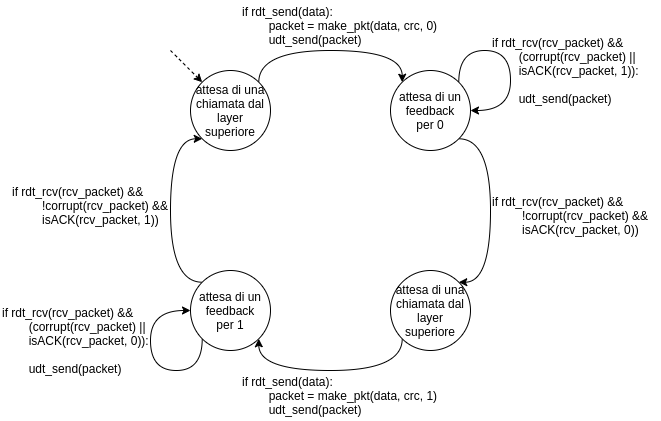
\includegraphics[width=340px]{images/3_Reti_connessione_diretta/rdt_2.2_sender.png}
    \caption{RDT 2.2 sender}
\end{figure}

\begin{figure}[H]
    \centering
    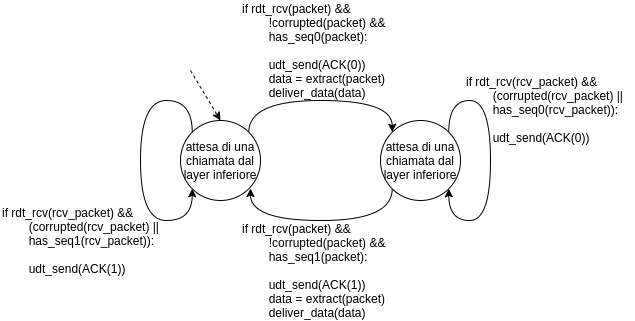
\includegraphics[width=340px]{images/3_Reti_connessione_diretta/rdt_2.2_receiver.png}
    \caption{RDT 2.2 receiver}
\end{figure}
Il ricevitore è visibilmente semplificato.

\subsubsection{RDT 3.0: canale con errori e perdite di pacchetti}
Su una connessione nella quale posso perdere dei pacchetti la detection degli errori ed il sequence\_number non sono abbastanza per risolvere tutte le problematiche.
Non possiamo accorgerci direttamente della perdita di un pacchetto, quindi come tattica usiamo quella dell' attesa dell'ACK, se l'ACK non arriva entro un tempo ragionevole allora re-inviamo il pacchetto.
Affinché funzioni tutto serve quindi un timer per contare il tempo passato dall' ultimo pacchetto inviato ed anche qui il ricevitore deve aggiungere all' ACK il sequence\_number.

La questione principale da porsi adesso è quanto tempo bisogna aspettare prima di dichiarare il timeout: troppo poco e si rischia di inondare la rete di duplicati evitabili, troppo lungo e l' efficienza della trasmissione ne risente pesantemente.
Il tempo andrebbe scelto leggermente maggiore del RTT.
\begin{figure}[H]
    \centering
    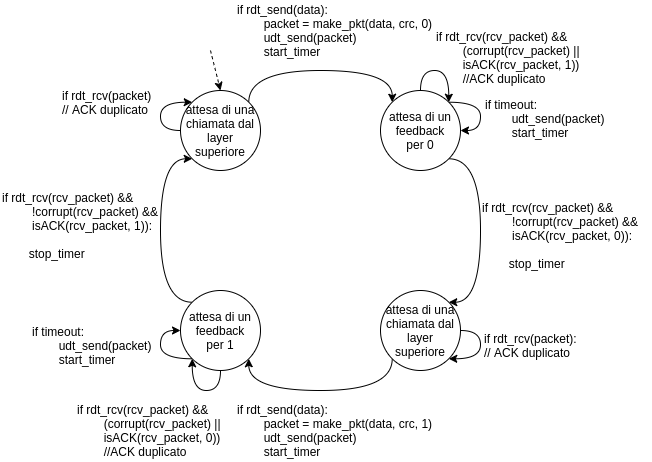
\includegraphics[width=340px]{images/3_Reti_connessione_diretta/rdt_3.0_sender.png}
    \caption{RDT 3.0 sender}
\end{figure}

\begin{figure}[H]
    \centering
    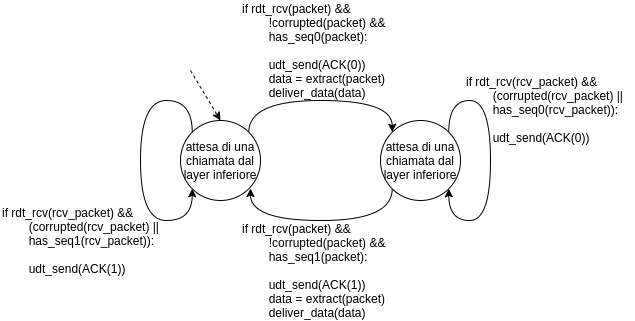
\includegraphics[width=340px]{images/3_Reti_connessione_diretta/rdt_2.2_receiver.png}
    \caption{RDT 3.0 receiver}
\end{figure}

\subsection{Alternative allo stop-and-wait}
L' algoritmo visto è funzionante, tuttavia le performance sono molto scarse.
L' utilizzo del mezzo di comunicazione è bassissimo in quanto per ogni pacchetto inviato attendiamo che arrivi e che ci torni una conferma:

Es: link da 1Gbps, 15ms di propagazione, pacchetti da 8000bit: il delay di trasmissione è:
$$ d_{trans} = \frac{L}{R} = \frac{8000 bits}{10^9 bps} = 8 ms $$
l' utilizzo del mezzo è invece:
$$ U_{sender} = \frac{\frac{L}{R}}{RTT + \frac{L}{R}} = 0.00027 $$
Ci metto 30ms per inviare 1KB di dati, per un throughput di 267Kbps su un link che ne ammette 1Gbps.

Il problema risiede nell' utilizzo dell' approcio stop-and-wait, il tempo in attesa è tempo morto!

\subsubsection{Pipelining}
Un approccio migliore sarebbe quello di inviare più pacchetti in sequenza ed aspettare diversi ACK in risposta:
\begin{figure}[H]
    \centering
    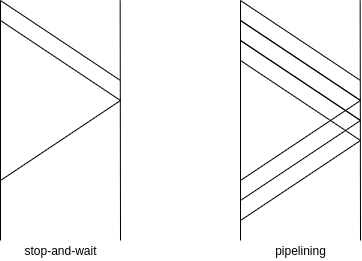
\includegraphics[width=200px]{images/3_Reti_connessione_diretta/stop-and-wait_pipelining.png}
\end{figure}

Per ottenere la pipeline bisogna apportare alcune modifiche al protocollo che abbiamo scritto:
\begin{itemize}
    \item bisogna avere delle sequenze più lunghe in quanto ci servono necessariamente più di 2 sequenze valide
    \item il trasmettitore e/o il ricevitore devono implementare meccanismi di buffering:
    \begin{itemize}
        \item il trasmettitore deve mantenere in memoria tutti i pacchetti che non hanno ancora ricevuto una conferma
        \item il ricevitore potrebbe implementare algoritmi di ri-ordinamento dei pacchetti out-of-order
    \end{itemize}
\end{itemize}
Possiamo avere due strategie di trasmissione:
\begin{itemize}
    \item Go-back-N
    \item Selective Repeat
\end{itemize}

\subsubsection{Go-back-N}
Il trasmettitore tiene in memoria una coda di pacchetti che non sono ancora stati confermati, i primi $N$ di questa lista formano la \emph{finestra}: quando invia pacchetti invia i pacchetti della finestra uno dopo l' altro in successione (in burst).

Quando il ricevitore li riceve invia un \emph{ACK cumulativo} cioè invia un ACK per l' ultimo pacchetto ricevuto correttamente in sequenza, non può inviare l' ACK per un pacchetto se non ha ricevuto correttamente anche tutti i precedenti, non possono esserci buchi.

Il trasmettitore mantiene un singolo timer per il pacchetto non confermato più vecchio, allo scadere di questo timer procede a reinviare la finestra a partire dal primo non confermato.
La finestra si sposta in avanti ogni volta che riceve un ACK per un pacchetto non ancora confermato.
Possono esserci ACK duplicati in quanto, appunto, se un pacchetto viene ricevuto corrotto il ricevitore provvederà ad inviare l' ACK dell'ultimo ricevuto correttamente.
\begin{figure}[H]
    \centering
    
\includegraphics[width=340px]{images/3_Reti_connessione_diretta/go-back-n_sender.png}
    \caption{Go-back-N sender}
\end{figure}
\begin{itemize}
    \item All' avvio la finestra parte dall' indice 1 ed il prossimo sequence\_number è uguale alla base in quanto non abbiamo pacchetti.
    Si noti che lasciamo lo 0 libero in modo che il ricevitore possa fare acknowledge su 0 per segnalare di non aver ricevuto il primissimo pacchetto.
    
    \item Alla chiamata dal layer superiore se la finestra non è piena provvediamo a creare un nuovo pacchetto con i dati da inviare e lo inviamo.
    Se la finestra era vuota, e quindi siamo al primo pacchetto della finestra, facciamo anche partire il timer.
    Se non c'è spazio nella finestra neghiamo la richiesta
    
    \item Se scatta il timer provvediamo a reinviare tutti i pacchetti nella finestra corrente
    
    \item Se riceviamo un pacchetto corrotto semplicemente non facciamo nulla
    
    \item Se riceviamo un pacchetto e non è corrotto usiamo il suo sequence\_number come nuova base della finestra, se coincide con la fine allora stoppiamo il timer, altrimenti lo facciamo ripartire in modo che adesso conti rispetto al pacchetto che ora è diventato il primo della finestra
\end{itemize}

\begin{figure}[H]
    \centering
    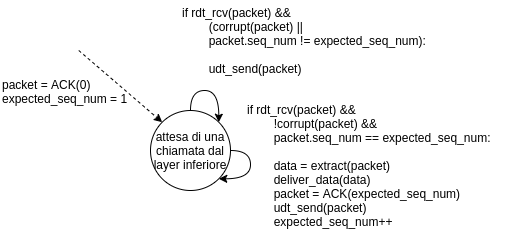
\includegraphics[width=340px]{images/3_Reti_connessione_diretta/go-back-n_receiver.png}
    \caption{Go-back-N receiver}
\end{figure}
\begin{itemize}
    \item All' avvio facciamo finta che l' ultimo pacchetto ricevuto avesse sequence\_number 0, quindi prepariamo il pacchetto di ACK su 0 mentre ci aspettiamo di ricevere il pacchetto con sequence\_number 1

    \item Se ricevo un pacchetto ed è corrotto o ha sequence\_number diverso da quello che mi aspetto provvedo a reinviare l' ultimo ACK prodotto
    
    \item Se ricevo un pacchetto non corrotto e con lo stesso sequence\_number che mi aspetto estraggo e consegno i dati che trasportava, creo l' ACK per quel sequence\_number e lo invio
\end{itemize}

Questo approccio ci permette di spostare la gran parte della complessità della trasmissione al trasmettitore, che infatti è più complesso, mentre lasciamo il minimo indispensabile al ricevitore.
In particolare questa implementazione non necessita nemmeno che il ricevitore abbia un buffer in quanto riceverà i pacchetti sempre nell' ordine corretto, se così non dovesse essere semplicemente verranno ignorati.

Questo approccio porta ad una grande ritrasmissione di pacchetti che magari sono arrivati correttamente ma ignorati in quanto out-of-order.


\subsubsection{Selective Repeat}
Il trasmettitore ha una coda di pacchetti che invia in sequenza (burst), riceve degli ACK per i singoli pacchetti e provvede a cancellare i pacchetti confermati da questa coda per far spazio ad altri.
Quando il timeout scade re-invia solo i pacchetti non confermati.

Il ricevitore quindi deve rispondere con i singoli ACK per i singoli pacchetti, deve anche avere un buffer interno in modo da mantere in memoria i pacchetti out-of-order per consegnarli al layer superiore nell' ordine corretto.

Anche in questo algoritmo possiamo pensare ad un concetto di finestra, per il trasmettitore la finestra parte dal primo pacchetto non confermato e va avanti per $N$ pacchetti.
In questo caso la finestra può avere dei buchi in quanto potrebbero esserci dei pacchetti di mezzo confermati ed altri no.

Anche il ricevitore ha un concetto di finestra che parte dal primo pacchetto che si aspetta di ricevere e va avanti per una dimensione $N$.
Se riceve un pacchetto che ha sequence\_number uguale a quello della base della finestra il contenuto viene subito spedito al layer superiore, altrimenti viene immagazzinato fino a che tutti i pacchetti prima di lui saranno ricevuti correttamente e spediti al layer superiore.


Queste due finestre saranno certamente \emph{out-of-sync} in quanto non sono concordate, questo potrebbe creare dei problemi se non tariamo bene le dimensioni del buffer e della finestra stessa:
\begin{figure}[H]
    \centering
    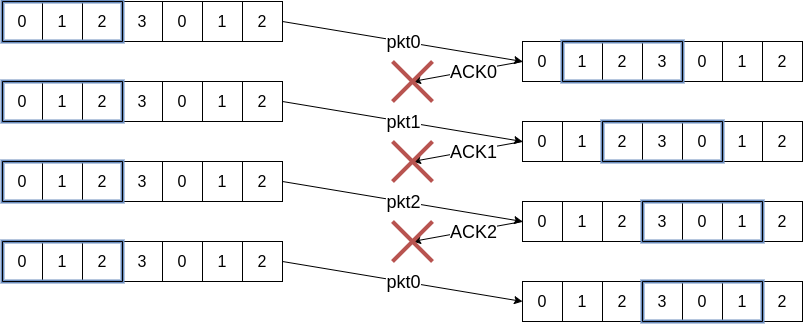
\includegraphics[width=300px]{images/3_Reti_connessione_diretta/window-desync.png}
\end{figure}
Supponiamo di avere la finestra di 3 elementi e di avere 4 sequence\_number:
\begin{itemize}
    \item TX invia il pacchetto 0, 1, 2
    \item RX riceve i pacchetti 0, 1, 2, risponde con gli ACK relativi e sposta la finestra
    \item Tutti gli ACK si perdono quindi TX non muove la sua finestra
    \item TX re-invia il pacchetto 0
    \item RX avendo la finestra spostata pensa che i pacchetti siano consecutivi e spedisce al layer superiore dei dati duplicati 
\end{itemize}

La dimensione della finestra deve quindi essere minore o uguale alla metà del numero dei sequence\_number che prevede la comunicazione.
Inoltre la larghezza della finestra dovrebbe evitare che il ricevitore debba memorizzare più pacchetti di quelli che effettivamente può memorizzare.
Possiamo scegliere un numero in base al RTT ed alla dimensione del buffer del ricevitore.

\subsection{Point to Point Protocol - PPP}
I Point to Point Data-Link protocols sono protocolli che permettono la comunicazione tra due elementi, un mittente ed un destinatario, connessi direttamente.
Alcuni esempi sono le linee ADSL e le connessioni dialup.
Tra questi il più utilizzato è stato il PPP, esso prevede:
\begin{itemize}
    \item \emph{Packet framing}: incapsula i datagrammi del livello rete in frame del livello data-link.
    Permette di trasportare tutti i protocolli di tipo rete, non solo IP, allo stesso tempo e di eseguire il demultiplexing verso il layer più alto.
    
    \item \emph{Bit transparency}: permette di trasportare nel frame qualsiasi pattern di bit
    
    \item Implementa la error detection ma non la correction
    
    \item \emph{Connection liveness}: si accorge e segnala al layer di rete se ci sono problemi sul collegamento
    
    \item \emph{network layer address negotiation}: gli endpoint possono mettersi d' accordo l' un l' altro per configurare i propri indirizzi di rete
\end{itemize}

Si noti che la mancanza di error recovery, flow control e data re-ordering può essere risolta implementandoli nei layer più in alto. 

\subsubsection{PPP Data frame}
Il frame del protocollo PPP è così composto:
\begin{figure}[H]
    \centering
    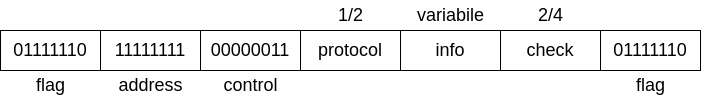
\includegraphics[width=300px]{images/3_Reti_connessione_diretta/ppp_data_frame.png}
\end{figure}
\begin{itemize}
    \item \emph{flag}: è il delimitatore del frame, si pone sia all' inizio che alla fine
    \item \emph{address}: è un campo inutilizzato che ha solo una possibile opzione
    \item \emph{control}: è un campo inutilizzato lasciato per futuri utilizzi
    \item \emph{protocol}: usato per specificare a quale protocollo di rete appartiene il frame
    \item \emph{info}: sono i dati da trasportare
    \item \emph{check}: CRC per la error detection
\end{itemize}

\subsubsection{Byte stuffing}
Dal momento che vogliamo poter trasmettere tutte le combinazioni di bit, per la data transparency, c'è bisogno di aggiustare la comunicazione affinché non ci siano problemi se nel campo info (ma non solo) dovesse comparire la sequenza del flag.
\begin{itemize}
    \item mittente: aggiunge la sequenza 01111101 prima di ogni byte flag
    
    \item destinatario: quando riceve la sequenza 01111101-flag rimuove il byte di escape e restituisce il byte successivo
\end{itemize}
NB: se si dovesse trasmettere lo stesso byte di escape lo si inserisce due volte affinché la prima volta venga scartato mentre la seconda venga trasmesso.

\subsubsection{PPP Link Control}
Prima di partire con la trasmissione dei dati i due endpoint possono negoziare alcune configurazioni:
\begin{itemize}
    \item configurazione del link PPP come la massima dimensione del frame ed un metodo di autenticazione, omissione dei campi address e control, ed altri.
    Questo viene fatto tramite il Link Control Protocol - LCP
    
    \item configurazione di rete come scambio e configurazione degli indirizzi IP
\end{itemize}


\subsection{Protocolli ad accesso multiplo}
Se volessimo interconnettere $N$ host differenti usando connessioni PPP avremmo necessità di $\frac{N(N-1)}{2}$ connessioni differenti.
Inoltre ogni host dovrebbe avere $N-1$ ingressi per il media, non è una soluzione che scala.
Per risolvere questo problema sono stati inventati i link ad accesso multiplo cioè dei media che sono condivisi tra più di 2 host.
Alcuni esempi sono il vecchio protocollo Ethernet ed il WiFi 802.11.

Per trasmettere bisogna darsi delle regole perché se due o più trasmissioni avvengono simultaneamente si ha una \emph{collisione} e quindi non si riceveranno dati corretti.
Il protocollo di accesso multiplo ideale dovrebbe prevedere:
\begin{itemize}
    \item pieno utilizzo: se solo un nodo vuole trasmettere esso deve poter trasmette alla massima capacità del canale
    \item fairness: se $M$ nodi vogliono trasmettere devono poterlo fare ad un rateo $\frac{R}{M}$
    \item completa decentralizzazione: non ci dovrebbero essere nodi speciali a coordinare la trasmissione
    \item semplicità
\end{itemize}

Abbiamo 3 classi di protocolli di accesso al mezzo:
\begin{itemize}
    \item a partizionamento del canale: si divide il canale in "pezzi" più piccoli, ad esempio in slot temporali, in canali di frequenza o su codice

    \item ad accesso casuale: il canale non è suddiviso, le collisioni sono ammesse ma si implementano dei meccanismi di recovery dalle collisioni.
    Quando un canale deve trasmettere trasmette a piena velocità.
    
    \item a turni: i nodi seguono un ordine ed attendono il loro turno per trasmettere, i nodi che hanno più da inviare prendono turni più lunghi
\end{itemize}

\subsubsection{TDMA - Time Division Multiple Access}
Si accede al media a turno, ogni stazione ha uno slot temporale di durata ben definita, di solito uguale al tempo di invio di un pacchetto.
Se una stazione non ha da trasmettere passa il suo slot in idle, quindi non si ha la fully utilization però si ha la fairness.
Non abbiamo una completa decentralizzazione in quanto serve qualcuno che dia l' ordine alle stazioni e dia la sincronizzazione.

\subsubsection{FDMA - Frequency Division Multiple Access}
Lo spettro del canale si suddivide in varie bande di frequenza, ad ogni stazione viene assegnato un singolo canale, se una stazione non ha da trasmettere rimane in idle sul suo canale.
Anche qui non abbiamo la fully utilization né la completa decentralizzazione, però è fair.

\subsubsection{CDMA - Code Division Multiple Access}
Ad ogni coppia di nodi viene assegnato un codice univoco per la trasmissione.
Tutte le comunicazioni avvengono simultaneamente ed ogni ricevitore può decodificare solo quella a lui destinata.
Permette la fully utilization e la fairness ma non è semplice.

\subsubsection{Slotted ALOHA}
Assumiamo che tutti i frame siano della stessa dimensione, dividiamo quindi il tempo in slot di dimensioni identiche a quelle necessarie per trasmettere un frame.
Quando un nodo ha dati da trasmettere lo fa all' inizio del primo slot temporale possibile, se 2 o più nodi trasmettono nello stesso slot tutti i nodi rilevano la collisione.
Quando ciò succede i nodi scelgono se provare a reinviare i frame nello slot successivo, scelgono casualmente di ritrasmettere con probabilità $p$, questa estrazione viene eseguita finché non riescono ad inviare i dati senza collisioni.
\begin{figure}[H]
    \centering
    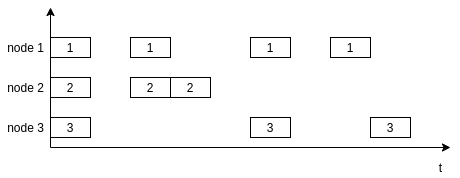
\includegraphics[width=250px]{images/3_Reti_connessione_diretta/slotted_aloha.png}
\end{figure}
In questa simulazione abbiamo 3 nodi che vogliono trasmettere e provano nel primo slot, essendoci una collisione devono tutti e 3 ritrasmettere.
Nello slot successivo nessuno dei 3 estrae la ritrasmissione, nel terzo slot ci riprovano 1 e 2 ma ancora una volta c'è una collisione.
Nel quarto slot finalmente il nodo 2 riesce a trasmettere da solo quindi il pacchetto viene consegnato intero, nessuna collisione.
Si continua così finché tutti e 3 non riescono a trasmettere da soli.

Tra i pro di questo algoritmo abbiamo:
\begin{itemize}
    \item se il nodo attivo è uno solo può trasmettere in ogni slot temporale, quindi utilizzo totale del mezzo
    \item alta decentralizzazione, l' unica cosa da negoziare è la durata di uno slot e l' inizio di ogni slot
    \item è semplice
\end{itemize}
tra i contro invece abbiamo:
\begin{itemize}
    \item ci sono tante collisioni quindi c'è tanto spreco di tempo
    \item in alcuni slot i nodi che vorrebbero trasmettere non lo fanno
    \item i nodi potrebbero detectare la collisione ben prima di finire di trasmettere i dati ma non lo fanno
    \item c'è da sincronizzarsi per avere tutti gli stessi slot
\end{itemize}

Calcoliamo l'efficienza: supponiamo che ci siano $N$ nodi con un po' di frame da inviare, ogni nodo trasmette in uno slot con probabilità $p$ uguale per tutti.
La probabilità che un nodo riesca a trasmettere correttamente in un frame è la probabilità che lui trasmetta $p$ e che tutti gli altri nodi non trasmettano $(1-p)^{N-1}$ quindi: $p(1-p)^{N-1}$.
La probabilità che qualsiasi nodo abbia successo è pertanto $Np(1-p)^{N-1}$.
La massima efficienza si ha con il $p*$ che massimizza $Np*(1-p*)^{N-1}$.
Per un numero alto di nodi eseguiamo il limite per $N \xrightarrow{} \infty$ ed otteniamo che l'efficienza massima è $\frac{1}{e} = 0.37$.
Si ha quindi una efficienza del canale del 37\%.

\subsubsection{Pure (unslotted) ALOHA}
La versione unslotted è più semplice, prevede l' eliminazione della sincronizzazione quindi si trasmette appena si hanno dei dati da trasmettere.
La probabilità di avere delle collisioni è quindi maggiore in quanto un frame inviato al tempo $t_0$ può collidere con i frame inviati nella finestra [$t_0-1$, $t_0+1$].

La probabilità di avere una comunicazione corretta è quindi la probabilità di essere gli unici che trasmettono nelle finestre [$t_0-1$, $t_0$], [$t_0$, $t_0+1$] cioè: $p(1-p)^{N-1}(1-p)^{N-1} = p(1-p)^{2(N-1)}$ per una efficienza massima di $\frac{1}{2e} = 0.18$

\subsubsection{CSMA - Carrier Sense Multiple Access}
Prima di trasmettere si ascolta il media, se c'è qualcuno che sta trasmettendo aspetto, altrimenti trasmetto tutto il frame.
Le collisioni continuano a verificarsi in quanto il tempo di propagazione ci offre una finestra di tempo nella quale possiamo ascoltare il mezzo, non sentire nulla e quindi iniziare la trasmissione, salvo poi accorgersi di avere una collisione.
In questo caso l' intero tempo della trasmissione del pacchetto è sprecato.

\subsubsection{CSMA/CD - Carrier Sense Multiple Access with Collision Detection}
Si usa la stessa tattica del CSMA ma quando si rileva una collisione si smette di trasmettere in modo da liberare il canale subito e non sprecare tempo.
La detection delle collisioni può essere eseguita in vari modi:
\begin{itemize}
    \item nelle reti su cavo si può misurare la potenza del segnale sul canale, se è maggiore della potenza che noi stiamo trasmettendo allora si ha una collisione
    
    \item anche nelle reti wireless si può usare la potenza del segnale tuttavia è più complesso in quanto entrano in mezzo anche le interferenze elettromagnetiche
\end{itemize}

Quando ci si accorge di una collisione si aumenta la potenza della trasmissione in modo da far accorgere prima anche gli altri nodi che stanno trasmettendo, questo si chiama \emph{jam signal}.

CSMA e la sua versione con CD garantisce la fullfilness in quanto possiamo trasmettere a pieno se siamo gli unici a dover trasmettere, è fair in quanto quando si incappa in una collisione ogni endpoint estrae un tempo casuale da attendere e quindi ci si da una specie di ordinamento permettendo comunque a tutti di trasmettere.
E' completamente decentralizzato in quanto nessun nodo ha più potere degli altri e non c'è una sincronizzazione.

Per bassi carichi è estremamente efficiente, tuttavia se il numero di host aumenta la sua efficienza cala drasticamente in quanto le collisioni aumentano.

\subsubsection{Polling}
E' un protocollo a turni in cui un nodo fa da \emph{master} e si occupa di interrogare i singoli nodi in sequenza chiedendo chi ha da trasmettere e dando singolarmente il permesso ad usare il media.

Essendo centralizzato abbiamo un single point of failure nel master, inoltre abbiamo un overhead perché il master deve interrogare singolarmente i nodi e dare loro il permesso.
Ogni nodo rileva una certa latenza perché deve aspettare di essere interrogato dal master prima di poter inviare.

\subsubsection{Token passing}
In una rete ad anello possiamo immaginare di avere un pacchetto che ci si passa tra gli host, chi ce lo ha in quel momento può trasmettere se ha pacchetti altrimenti provvede a passare in avanti il token.
E' come moderare un dibattito permettendo solo a chi ha il microfono in quel momento di parlare.

Non abbiamo single point of failure in quanto il token viene passato nella rete da un nodo all' altro e non ci sono nodi più importanti degli altri.

Abbiamo un overhead dettato dal passaggio del token ed anche una latenza in quanto devo aspettare di avere il token prima di poter trasmettere.

\subsection{Indirizzamento}
Per permettere ai protocolli ad accesso multiplo di funzionare e creare l' astrazione di connessioni punto-punto abbiamo la necessità di aggiungere un indirizzamento.
Ogni host ha un proprio indirizzo ed i frame che transitano nella rete riportano gli indirizzi del mittente e del destinatario.

Quando un host trasmette tutti gli altri ascoltano ma se non sono i diretti interessati droppano il pacchetto.

L' indirizzo è associato univocamente alla Network Interface Card dalla casa produttrice ed è un indirizzo su 48 bit (MAC address).
E' anche detto \emph{physical address}, \emph{link-layer address}.

Oltre ad un indirizzo univoco per ogni host prevediamo anche un indirizzo di \emph{broadcast} cioè un indirizzo che indica che tutti sono interessati a ricevere il messaggio.

\subsection{Local Area Network - LAN}
Sono reti che hanno la copertura di un edificio, una sua parte o alcuni edifici vicini geograficamente.
L' accesso è eseguito tramite Medium Access Control Protocol quindi media condivisi e si usa un indirizzamento basato su indirizzi fisici (MAC).
In generale le velocità vanno dai 10Mbps ai 10Gbps.

\subsubsection{Topologia delle LAN}
Possiamo avere diverse tipologie, le più comuni sono state:
\begin{figure}[H]
    \centering
    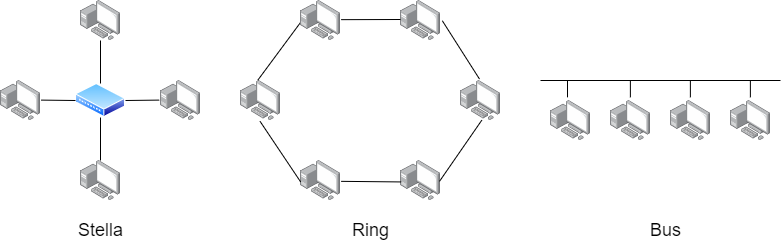
\includegraphics[width=330px]{images/3_Reti_connessione_diretta/network_topologies.png}
\end{figure}
NB: nella topologia a bus per evitare la riflessione del segnale si inserisce un resistore da $50 \Omega$ alla fine del cavo.

NB: la topologia a stella con un hub al centro non è altro che una topologia a bus in quanto l' hub si occupa di ripetere sugli altri canali ciò che riceve da uno singolo, per questo la stella è anche detta \emph{folded hub}.

\subsubsection{Indirizzi MAC}
Un indirizzo MAC è un indirizzo composto da 48 bit associato ad un adattatore di rete.
I primi 24 bit indicano il produttore dell' interfaccia di rete ed è assegnato dalla IEEE, gli ultimi 24 bit invece sono assegnati dal produttore alla singola interfaccia.

Per rappresentarli semplicemente si usa una notazione esadecimale.
Il MAC di broadcast è per convenzione FF:FF:FF:FF:FF:FF.

Questi indirizzi sono pertanto univocamente associati e sono portabili attraverso le diverse reti a differenza degli indirizzi IP che hanno senso solo in una rete.

\subsection{Ethernet}
E' la tecnologia di accesso tramite cavo più utilizzata oggigiorno, è economica, semplice da utilizzare e permette di avere velocità tra i 10Mbps ed i 10 Gbps.

\begin{figure}[H]
    \centering
    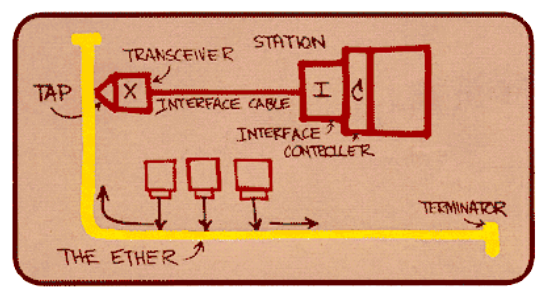
\includegraphics[width=200px]{images/3_Reti_connessione_diretta/Metcalfe_ethernet.png}
\end{figure}
In foto lo sketch dell'interfaccia di rete Ethernet pensata da Bob Metcalfe.

Nella topologia a bus abbiamo tutti gli host connessi ad un singolo bus e tutti gli host sono nello stesso dominio di collisione.

Nella topologia a stella invece ogni host ha un collegamento dedicato verso l' hub centrale ma essendo l' hub un ripetitore di segnale si continua ad avere un singolo dominio di collisione.

\subsubsection{Hub}
L' hub è un dispositivo di rete che lavora sul layer fisico, è banalmente un ripetitore di segnale: tutti i bit che arrivano in una interfaccia vengono ripetuti su tutte le altre interfacce alla stessa velocità di ingresso.
Questo significa che qualsiasi nodo connesso all' hub può collidere con tutti gli altri.
Non c'è un concetto di buffering, tantomeno un metodo di accesso CSMA/CD.

\subsubsection{Switched Star topology}
Oggigiorno si usano delle topologie a stella con al centro un apparato di rete chiamato \emph{switch}.
Questo dispositivo lavora al livello data-link quindi riesce a comprendere i protocolli di accesso ed i frame.
Permette anche di bufferizzare i frame in ingresso e di spedirli in uscita ai diretti interessati dopo aver controllato che il media sia libero e che quindi non ci sia il rischio di collisioni.
Permette inoltre di inviare il traffico direttamente al destinatario senza dover passare per una ripetizione in broadcast.

\subsubsection{Struttura di un frame ethernet}
\begin{figure}[H]
    \centering
    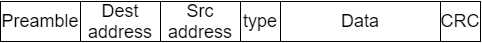
\includegraphics[width=250px]{images/3_Reti_connessione_diretta/ethernet_frame.png}
\end{figure}
\begin{itemize}
    \item preambolo: 7 byte con valore 10101010 ed 1 byte con valore 10101011, sono usati per sincronizzare la velocità del ricevitore con quella del trasmettitore
    
    \item indirizzo di destinazione: è il MAC address di chi deve ricevere il frame.
    E' inviato per primo in modo che chiunque stia ascoltando e non è il destinatario possa smettere di immagazinare i dati trasmessi
    
    \item indirizzo sorgente: è il MAC address di chi sta inviando il frame
    
    \item tipo: indica il protocollo di livello superiore al quale recapitare i dati incapsulati nel frame.
    Ora principalmente IP ma non è detto
    
    \item CRC: usati per l' error detecion del frame.
    Non fa error correction
\end{itemize}
Un frame ethernet è grande almeno 64byte, cioè 512 bit.

\subsubsection{Codifica Manchester}
Per trasmettere i dati sulla linea si utilizza la codifica manchester:
\begin{figure}[H]
    \centering
    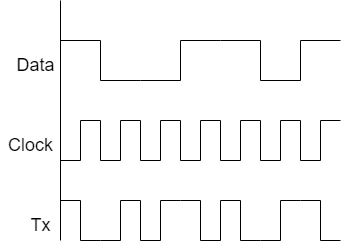
\includegraphics[width=220px]{images/3_Reti_connessione_diretta/manchester_encoding.png}
\end{figure}
il flusso dei dati viene xorato con il clock e si trasmette il risultato.
Questa codifica è utile in quanto permette ai clock del ricevitore e del trasmettitore di rimanere sincronizzati per tutta la durata della trasmissione, inoltre in ogni bit c'è una transizione dall' alto al basso o dal basso all' alto, quindi senza conoscere il centro dell' impulso per campionare possiamo rilevare questa transizione.

Per estrarre il clock dai dati il ricevitore utilizza un anello ad aggancio di fase.
Di fatto il preambolo è una porzione del frame di pertinenza del layer fisico.

\subsubsection{Proprietà del protocollo Ethernet}
Ethernet è un protocollo connectionless quindi non prevede un handshake iniziale, tantomeno una chiusura della connessione alla fine della trasmissione.

E' un protocollo non affidabile, non ci sono ACK né NAK, è un flusso continuo di datagrammi che possono anche avere dei gap.
Questa non affidabilità può essere poi aggiustata dai protocolli dei layer superiori.

Usa una politica CSMA/CD per l' accesso al mezzo.

\subsubsection{CSMA/CD di Ethernet}
\begin{itemize}
    \item La scheda di rete riceve dei dati dal layer di rete, crea un frame

    \item se la NIC rileva il canale libero per il tempo di 96 bit allora inizia la trasmissione del frame.
    Se il canale è occupato aspetta finché non riesce a vederlo libero per 96 bit time
    
    NB: quanto vale un bit time? Supponiamo di trasmettere ad 10Mbps allora $\frac{1}{10^{7}} = 0.1\mu s$
    
    \item se la NIC riesce ad inviare il frame completamente ha finito con quel frame
    
    \item se invece rileva una collisione durante la trasmissione abortisce ed invia 48 bit di segnale di disturbo in modo da far accorgere anche gli altri host che stanno trasmettendo
    
    \item dopo aver interrotto la trasmissione aspetta un \emph{exponential backoff} cioè all' n-esima collisione sceglie $K$ casualmente nell' insieme $\{0, 1, 2, \_, 2^{m}-1\}$ con $m=min(n, 10)$ ed aspetta per $K \cdot 512$ bit time per poi tornare ad ascoltare il mezzo per la trasmissione
\end{itemize}
L' exponential backoff è un metodo per adattarsi al carico di trasmissione del mezzo, se dopo un paio di tentativi continuo ad avere collisioni vuol dire che devo provare ad aspettare molto di più.

Dopo 17 collisioni successive il frame viene droppato direttamente.

\subsubsection{Standard Ethernet}
Ci sono diversi standard ethernet a diverse velocità e per diversi media fisici:
\begin{figure}[H]
    \centering
    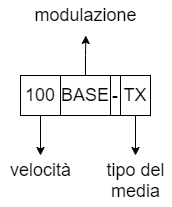
\includegraphics[width=100px]{images/3_Reti_connessione_diretta/standard_ethernet.png}
\end{figure}
